%%%%%%%%%%%%%%%%%%%%%%%%%%%%%%%%%%%%%%%%%%%%%%%%%%%%%%%%%%%%%%%%%%%%%%
% LaTeX Template: Beamer arrows
%
% Source: http://www.texample.net/
% Feel free to distribute this template, but please keep the
% referal to TeXample.net.
% Date: Nov 2006
% 
%%%%%%%%%%%%%%%%%%%%%%%%%%%%%%%%%%%%%%%%%%%%%%%%%%%%%%%%%%%%%%%%%%%%%%
% How to use writeLaTeX: 
%
% You edit the source code here on the left, and the preview on the
% right shows you the result within a few seconds.
%
% Bookmark this page and share the URL with your co-authors. They can
% edit at the same time!
%
% You can upload figures, bibliographies, custom classes and
% styles using the files menu.
%
% If you're new to LaTeX, the wikibook is a great place to start:
% http://en.wikibooks.org/wiki/LaTeX
%
%%%%%%%%%%%%%%%%%%%%%%%%%%%%%%%%%%%%%%%%%%%%%%%%%%%%%%%%%%%%%%%%%%%%%%

\documentclass[9pt]{beamer} %
\usetheme{CambridgeUS}
\usepackage[utf8]{inputenc}
\usefonttheme{professionalfonts}
\usepackage{times}
\usepackage{tikz}
\usepackage{amsmath}
\usepackage{verbatim}
\usetikzlibrary{arrows,shapes}
\usepackage{framed, color}
\definecolor{shadecolor}{rgb}{0.690, 0.933, 0.525}

\author{Daniel López García\\ Lothar Soto Palma\\ Elena María Toro Pérez\\\textit{Universidad de Granada}}
\title{Historia de las matemáticas\\ Machine Learning}

\begin{document}

% For every picture that defines or uses external nodes, you'll have to
% apply the 'remember picture' style. To avoid some typing, we'll apply
% the style to all pictures.
\tikzstyle{every picture}+=[remember picture]

% By default all math in TikZ nodes are set in inline mode. Change this to
% displaystyle so that we don't get small fractions.
\everymath{\displaystyle}

\begin{frame}
\titlepage
\end{frame}

\begin{frame}
\frametitle{Índice}
\tableofcontents
\end{frame}

\section{Introducción}
	\begin{frame}
	\frametitle{Introducción}
    \textbf{Machine learning} es una disciplina científica del ámbito de la Inteligencia Artificial que crea sistemas que aprenden automáticamente.\\
	
	Hoy en día, podemos observar la aplicación concreta de Machine Learning en varios campos que nos rodean. Algunos de ellos son:
		\begin{itemize}
		    \item \textbf{Automóviles:} sistemas de piloto automático.
		    \item \textbf{Finanzas:} asesoría de préstamos (aceptación/denegación de un crédito).
		    \item \textbf{Internet:} compras on-line, anuncios on-line.
		    \item \textbf{Medicina:} diseño de prediagnósticos médicos basados en síntomas del paciente.
		    \item \textbf{Recursos Humanos:} predicción de qué empleados serán más rentables el año que viene.
		    \item \textbf{Transporte:} sistemas de rutas y seguimiento de flotas.
		\end{itemize}
	\end{frame}
	
	\begin{frame}
	\frametitle{Antecedentes Estadísticos}
	Para que los sistemas puedan aprender por ellos mismos, se utilizan una serie de técnicas y algoritmos capaces de crear modelos predictivos, patrones de comportamiento, etc.\\
	
	Todo este proceso está basado en la teoría estadística.\\
	
	
	Los 3 métodos más importantes son:
	\begin{itemize}
	    \item \textbf{Teorema de Bayes.}
	    \item \textbf{Método de los mínimos cuadrados.}
	    \item \textbf{Cadenas de Markov.}
	\end{itemize}
	\end{frame}
	
		\begin{frame}
	\frametitle{Un ejemplo ilustrativo}
	\begin{shaded}
	Una empresa de telefonía quiere saber qué clientes están en “peligro” de darse de baja de sus servicios para evitar que se vayan a la competencia.
	\begin{itemize}
	    \item La empresa tiene \textbf{muchos datos} de los clientes, pero seguramente los usa solo para facturar y para hacer estadísticas.
	    \item Esta cantidad inmensa de datos son \textbf{imposibles de analizar por una persona} para sacar conclusiones y menos aún para hacer predicciones.
	    \item Los \textbf{algoritmos} en cambio sí pueden detectar patrones de comportamiento contando con las variables que le proporcionamos y descubrir cuáles son las que le han llevado, en este caso, a darse de baja como cliente.
	\end{itemize}
	\end{shaded}
	\end{frame}
	
	    \begin{frame}
	\frametitle{Un ejemplo ilustrativo}
	\begin{figure}[H]
    \centering
    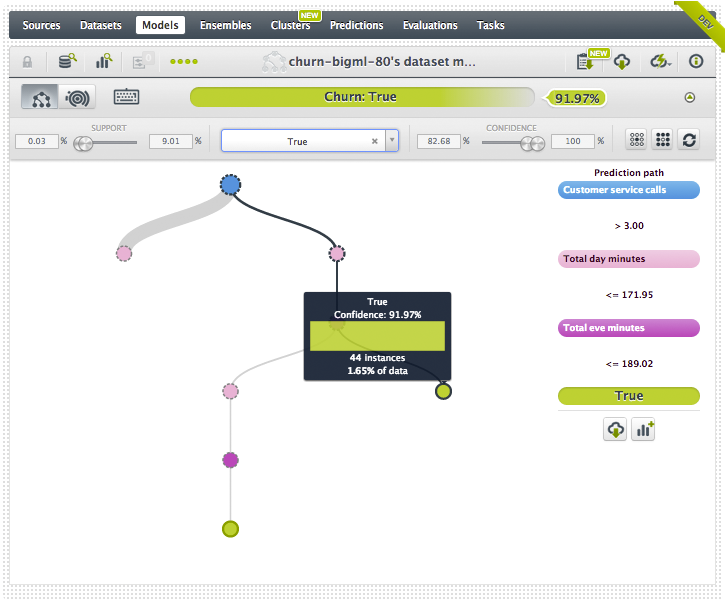
\includegraphics[width=0.650\textwidth]{ejemploMachineLearning.png}
    \caption{Ejemplo de una predicción de una compañía de telefonía ficticia}
    \end{figure}
	
	\end{frame}
	
	\section{Tipos de aprendizaje}
	\begin{frame}
	\frametitle{Tipos de aprendizaje}
	Las diferentes formas de aprender se pueden clasificar en función de la salida que produzcan y de su forma de tratar con los ejemplos. Los principales tipos son:
\begin{itemize}
	\item \textbf{Aprendizaje supervisado:} se conoce a priori una clasificación de los datos del problema.
	\item \textbf{Aprendizaje no supervisado}: no se tiene conocimiento a priori sobre el problema, no hay instancias etiquetadas.
	\item \textbf{Aprendizaje semisupervisado}: estos algoritmos combinan los dos algoritmos anteriores (se tienen en cuenta ejemplos clasificados y no clasificados).
	\item \textbf{Aprendizaje por refuerzo}: el sistema aprende a base de prueba-error, reforzando las acciones que reciben una respuesta positiva.
	\item \textbf{Aprendizaje multi-tarea}: métodos que usan conocimiento previamente aprendido para resolver problemas parecidos.
\end{itemize}
	\end{frame}
	
\section{Una idea inicial}
	\begin{frame}
	\frametitle{Una idea inicial}
	En \textbf{1950}, Alan Turing publicó uno de sus artículos más importantes para la revista \textit{Mind} donde propuso \textbf{el Test de Turing}.\\
	
	Se basa en una hipótesis: ``si una máquina se comporta en todos los aspectos como inteligente, entonces, dicha máquina debe ser inteligente''.\\

    El artículo de Turing comenzaba con una frase que era toda una declaración de intenciones de lo que evaluaría el test:
    \begin{shaded}
    "Propongo considerar la siguiente cuestión: ¿Pueden pensar las máquinas?"
    \end{shaded}
    
    Por lo que el resultado que se obtiene de este test es \textbf{intentar medir si una máquina puede ser inteligente} con un método que, aún hoy, sigue estando vigente.\\
	\end{frame}
	
	\begin{frame}
	\frametitle{¿En qué consistía el Test de Turing?}
	\begin{itemize}
	    \item Se basaba en el Juego de la Imitación, en el cual se ubicaban en una habitación un \textbf{hombre} y a una \textbf{mujer} con terminales con algún sistema de comunicación. El objetivo del interrogador era descubrir quién era la mujer y quién era el hombre, mientras que el de los otros dos era convencer al interrogador de que son la mujer.
	    \item Turing proponía realizar un cambio: coger a uno de los dos sujetos y sustituirlo por una \textbf{máquina}. Así, cambiaba el objetivo de reconocer el sexo por el de reconocer la máquina.
	\end{itemize}
	
	\begin{figure}[H]
    \centering
    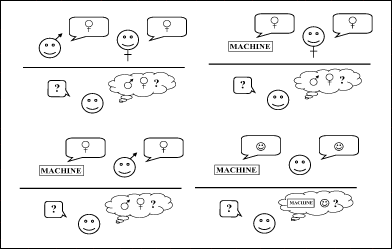
\includegraphics[width=0.45\textwidth]{testdeturing.PNG}
    \caption{Test de Turing}
    \label{Test de Turing}
    \end{figure}
	\end{frame}

\section{Problema de clasificación}
	\begin{frame}
	\frametitle{Problema de Clasificación}
		\begin{itemize}
			\item[] En el aprendizaje automático y la estadística en problema de las clasificación consiste en identificar un conjunto de categorías a la que pertenece una observación o conjunto de instancias de una población. La clasificación es un ejemplo de reconocimiento de patrones en una población. 
	
			\item[] \textbf{Conceptos previos}
	
			\begin{itemize}
				\item \textbf{Dato o instancia}: Los datos son representación simbólica de atributos o un conjunto de atributos, estos son la principal materia prima para el aprendizaje.
				\item \textbf{Conjunto de entrenamiento}:  Partición de un conjunto de datos que es usado para descubir relaciones en los datos que posteriormente nos puedan servir para predecir
				\item \textbf{Conjunto de prueba}: Partición de un conjunto de datos que se usa para evaluar el modelo generado usando el conjunto anterior.
			\end{itemize}
		\end{itemize}

	\end{frame}
			
	\begin{frame}
	\frametitle{Problemas de los métodos de clasificación}
	Uno los grandes problemas de los algoritmos de clasificación es el sobreajuste o sobreentrenamiento
		\begin{figure}[H]
			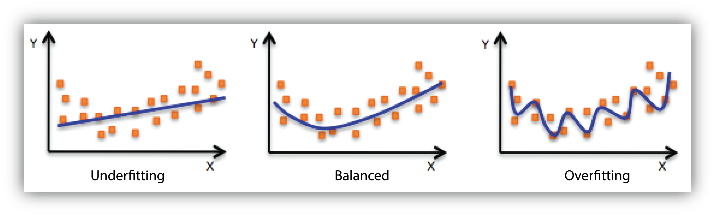
\includegraphics[scale=0.30]{overfitting.png} 
			\caption{Ejemplo de sobreajuste}
		\end{figure}
		\begin{itemize}
			\item \textbf{¿Cuándo se produce?}: Se produce cuando un modelo se ajusta muy bien al conjunto de datos que usamos para entrenar y que de alguna manera elimina la generalidad que debería de tener el modelo para poder tratar con él.
			\item \textbf{¿Cómo tratar de evitarlo?}: Una de las formas es la validación, es un conjunto de técnicas que se aplican normalmente antes de evaluar el modelo obtenido con el aprendizaje sobre un conjunto de entrenamiento y sirve para obtener resultados que ilustren una hipotética relación entre los atributos.
		\end{itemize}
	\end{frame}
	
	\begin{frame}
	\frametitle{Validación Cruzada}
		\begin{figure}[H]
		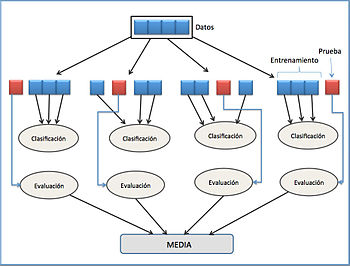
\includegraphics[scale=0.6]{5-fold} 
		\caption{Ejemplo de Validación cruzada}
	\end{figure}
	\end{frame}
	
	\subsection{Redes neuronales}
		
		\begin{frame}
		\frametitle{Red Neuronal}
		Las redes neuronales son un conjunto de neuronas artificiales interconectadas, son un paradigma de aprendizaje y procesamiento automático inspirado en el sistema nervioso, que es objeto de estudio en el campo de la inteligencia artificial.
		\begin{itemize}
		\item \textbf{¿Cuándo surgió esta idea?}
		\item \textbf{¿Qué ideas han dado lugar a las redes neuronales tal y como son en la actualidad?}
		\end{itemize}	
		\end{frame}
	
		\begin{frame}
		\frametitle{Marco histórico (Redes neuronales)}
			Los hechos más destacados:
			\begin{itemize}
				\item En el año \textbf{1943}, Warren McCulloch y Walter Pitts construyen un modelo simple de red neuronal usando circuitos electrónicos. 
				\item En el año \textbf{1949}, Donald Hebb introduce la teoría de la asamblea celular.
				\item En los años 50, Nathanial Rochester hizo un primer intento fallido de simular una red neuronal.
				\item En el año \textbf{1951}, Marvin Lee Minsky y Dean Edmonds construyen la primera máquina que ejecutaría una red neuronal.
				\item En el año \textbf{1958}, Frank Rosenblatt desarrolla el perceptrón.
			\end{itemize}
		\end{frame}	
	
		\begin{frame}
		\frametitle{Perceptrón}
Es un tipo de red neuronal artificial. El modelo más simple de un perceptrón es una neurona. 

Se pudo demostrar que el perceptrón era capaz de clasificar patrones correctamente.
		
	La mayor desventaja de este tipo de redes es su incapacidad para solucionar problemas que no sean linealmente separables.
		\begin{figure}
		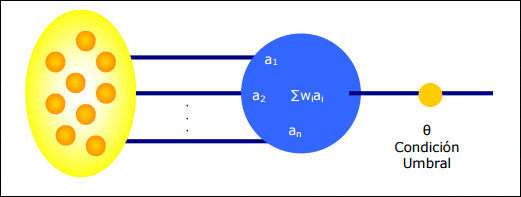
\includegraphics[scale=0.55]{Perceptron.PNG}
		\caption{Estructura del perceptrón.} 
		\end{figure}
		\end{frame}	
		
	\begin{frame}
	\frametitle{Modelo matematico del perceptron}
	\textit{Un \textbf{perceptrón simple} es un dispositivo de computación con umbral $\theta$ y $N$ entradas reales $x_1, ..., x_N$ a través de arcos con pesos $w_1, ..., w_N$ y que tiene salida $1$ cuando $\sum_{i}w_ix_i \geq \theta$ y $-1$ en caso contrario.}

Es decir, supongamos la función  de clasificación $f$ en $\mathbb{R}^n$ tal que:

\[
f(x_1, x_2, ..., x_N) = \left\{ \begin{array}{lcc}
             1 &   si  & w_1x_1 + w_2x_2 + ... + w_Nx_N \geq \theta \\
             \\ -1 &  si  &  w_1x_1 + w_2x_2 + ... + w_Nx_N < \theta
             \end{array}
   \right.
\]

Dicha función realiza una partición en el espacio $\mathbb{R}^n$ de patrones de entrada: por una parte estarían los patrones con salida $+1$ y por otra parte los patrones con salida $- 1$. Por lo tanto, diremos que la función f clasifica a los patrones de entrada en dos clases.

En este caso, se expresa la función $f$ mediante la función signo, es decir:
\[
f(x_1, x_2, ..., x_N) = sign(x_1, x_2, ..., x_N)
\]

donde la función signo es:
\[
sign(x_1, x_2, ..., x_N) = \left\{ \begin{array}{lcc}
             1 &   si  & x \geq 0 \\
             \\ -1 &  si  &  x < 0
             \end{array}
   \right.
\]
	\end{frame}
	\subsection{Vecino más cercano}
		\begin{frame}
		\frametitle{Vecino más cercano}
		\begin{itemize}
		\item El algoritmo de clasificación K-Nearest Neighbor o K-vecinos más cercanos es uno de los métodos de clasificación más fundamental y sencillo.
		\item Fue introducido en 1951 por Fix y Hodge para resolver el problema de clasificación.
		\item No fue hasta el año 1967 que este método no tuvo constancia.
		\item Este hito está considerado como el nacimiento del campo de reconocimiento de patrones en computadores.
		\item \textbf{¿Cómo es su funcionamieto?}
				\begin{figure}[H]
		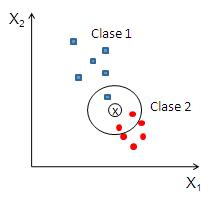
\includegraphics[scale=0.6]{ejemploKNN} 
		\caption{Ejemplo de Validación cruzada}
	\end{figure}
			\end{itemize}
		\end{frame}
	\subsection{Árboles de decisión}
		\begin{frame}
		\frametitle{Árboles de decisión}
		
		\end{frame}
	\subsection{SVM}
		\begin{frame}
		\frametitle{SVM}
		\end{frame}

\section{Otras técnicas para el aprendizaje}
	\begin{frame}
	\frametitle{Otras técnicas para el aprendizaje}
	\end{frame}

	\subsection{Clustering}
		\begin{frame}
		\frametitle{Clustering}
		\end{frame}

	\subsection{Algoritmos genéticos}
		\begin{frame}
		\frametitle{Algoritmos genéticos}
		\end{frame}

	\subsection{Colonias de hormigas}
		\begin{frame}
		\frametitle{Colonias de hormigas}
		\end{frame}

\section{Máquinas y juegos}
	\begin{frame}
	\frametitle{Máquinas y juegos}
	\end{frame}


\end{document}
              
            